\documentclass{standalone}

\usepackage{tikz}
\usepackage{pgfplots}

\definecolor{ggreen}{HTML}{666666}

\begin{document}
	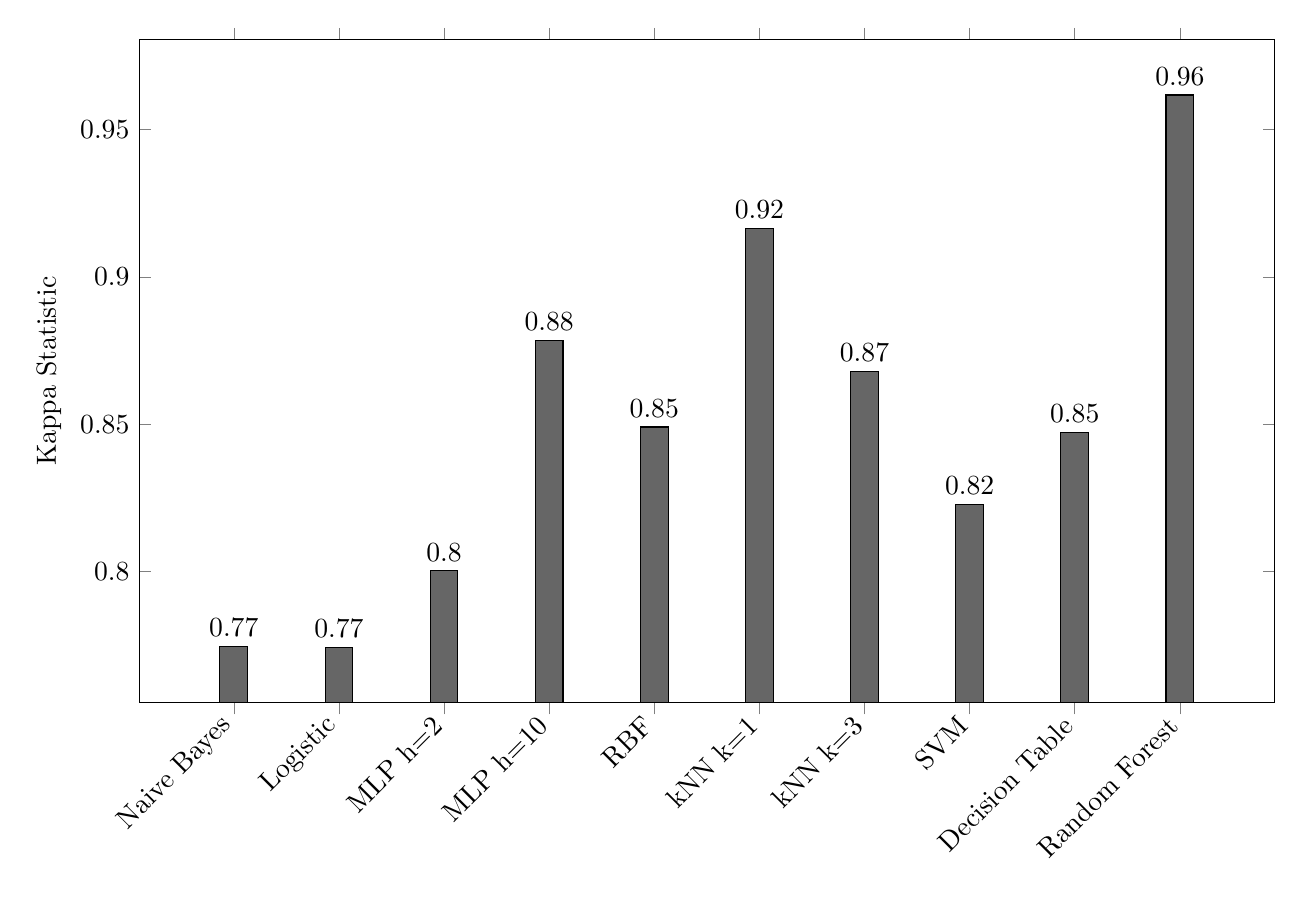
\begin{tikzpicture}
	\begin{axis}[
	ybar,
	width  = 16cm,
	height = 10cm,
	enlargelimits=0.10,
	legend style={at={(0.5,-0.2)},
		anchor=north,legend columns=-1},
	ylabel={Kappa Statistic},
	symbolic x coords={Naive Bayes, Logistic, MLP h=2, MLP h=10, RBF, kNN k=1, kNN k=3, SVM, Decision Table, Random Forest},
	xtick=data,
	nodes near coords, 
	nodes near coords align={vertical},
	x tick label style={rotate=45,anchor=east},
	]
	\addplot [style={black,fill=ggreen,mark=none}] coordinates {
			(Naive Bayes, 0.7746)
			(Logistic, 0.7743)
			(MLP h=2, 0.8003)
			(MLP h=10, 0.8784)
			(RBF, 0.8491)
			(kNN k=1, 0.9166)
			(kNN k=3, 0.8679)
			(SVM, 0.8229)
			(Decision Table, 0.8473)
			(Random Forest, 0.9618)
		};
	\end{axis}
	\end{tikzpicture}
\end{document}
